\NeedsTeXFormat{LaTeX2e}[1995/12/01]
\documentclass[10pt]{article}    

% Load packages
\usepackage{cite} % Make references as [1-4], not [1,2,3,4]
\usepackage{url}  % Formatting web addresses  
% \usepackage[utf8]{inputenc} %unicode support
\urlstyle{rm}
\usepackage{indentfirst}
%% \setlength{\doublerulesep}{\arrayrulewidth}
\usepackage{amsmath,amsfonts,amssymb}
\usepackage[pdftex, bookmarks, colorlinks]{hyperref}


%% \def\includegraphic{}
%% \def\includegraphics{}
\usepackage{color,graphicx}


\setlength{\topmargin}{0.0cm}
\setlength{\textheight}{21.5cm}
\setlength{\oddsidemargin}{0cm} 
\setlength{\textwidth}{16.5cm}
\setlength{\columnsep}{0.6cm}


\begin{document}


\title{Supplementary online material for ``An individual-based model
  simulator for transposable elements dynamics and evolution''}


\author{Felipe Figueiredo\footnote{philsf79@gmail.com} \and
  Claudio Struchiner }

%% \footnote{Programa de Pós-graduação em Biologia Computacional e
%%   Sistemas, Instituto Oswaldo Cruz, BCS/IOC/Fiocruz}
%% \footnote{Programa de Computação Científica, PROCC/Fiocruz}


\maketitle
\tableofcontents

%%%%%%%%%%%%%%%%%%
\section{Overview of the simulator}

%% Here we describe the overall structure of the simulator. More specific
%% details are available in the API documentation, provided with the
%% software.

The \verb|TRepid| simulator is an Object-Oriented system, with
individual hosts and TEs each represented by objects. It's main
interface with the user is provided by a plain-text configuration file
that should be present in directory of the simulation. The simulation
sub-directory tree will be created, and data and log files written by
the simulator as required.

\subsection{The main players}
\label{sec:main_players}

The main class defines simulation objects that contain all the
information and data related to a given simulation. Associated with
each simulation object is a configuration object to access or modify
any parameter of the simulation, including equations parameters, file
names, etc. It collects all configuration parameters and variables
from configuration files, or use defaults if values are not provided
by the user.




%\section{Usage of the simulator}

\subsection{Basic usage: Input}
The principal way of setting up a new simulation is through a
configuration file called \verb|trepid.conf|, inside which the user
defines parameters for all the models.

The default configuration file that comes with the simulator has all
parameters filled with default values, and comments explain what they
mean. This file is divided in sections to organize semantics for the
user. These categories are not interpreted though, since only variable
names are used and users are free to remove the section names and
define the config file in the order they prefer.

After preparing the configuration file, the user can run the
\verb|trepid| program inside the directory where the config file is
located. Upon starting, the simulator looks for the \verb|trepid.conf|
file, and if found, create a directory structure for the population
(even if the population is not saved at the end of the simulation), a
directory for logs and results, and finally a directory for the
Templates for the hosts with TEs.

The Templates dir is where one or more genome templates are located,
and used to create the GM (Genetically Modified, i.e. with TEs)
subpopulation. If the user wants t ouse a GM population, at least one
GM template must exist. If the templates directory is previously
non-existant, a GM population won't be created, and in this case the
simulator aborts.

If the configuration file is not found or is empty, default values
will be used for all parameters. The same happens to any parameter not
defined in the config file, if it is incomplete. The user can check
what parameters were set for each simulation in the log header.

\subsection{The default config file}
\label{sec:default_config}

In this section we describe all of the variables definable in the
confi file, showing the default values as illustration. These are the
parameters used for a very simple simulation of a Master Gene model in
a small host population that does not have generation overlap.

\subsection{General}
\label{sec:default_config_general}

{\bf Simulation time and initial subpopulations}

\begin{verbatim}
#####################################
[General]
# Number of generations (default: 10)
it_max = 10
\end{verbatim}

FIXME: include other general variables, save\_*, sample\_gm,
interactive, often\_max.

\subsection{Initial}
\label{sec:default_config_initial}

FIXME: include other initial variable: init\_gender .

\begin{verbatim}
#####################################
[Initial]
# Initial Susceptibles (default: 900)
S_0 = 0
# Initial Infectious (default: 100)
I_0 = 10000
# Initial Removed (default: 0)
R_0 = 0
\end{verbatim}

The parameter \verb$it_max$ determines how many iterations of the model,
i.e., how many generations will be simulated.

The $F_0$ population is determined by three initial subpopulations. In
these parameters, the notations inspired by the SIR epidemic model of
the early prototypes were maintained. \verb$S_0$ symbolizes the
initial wild subpopulation, \verb$I_0$ the initial GM subpopulation
(i.e. individuals that carry TEs) and \verb$R_0$ the Deceased or past
individuals.

If a population was previously saved to disk, the files wil be
automatically read and the $F_0$ population will be constructed using
those individuals. If the initial parameters for either of \verb$S_0$,
\verb$I_0$ and \verb$R_0$ are greater than the pre-existing
individuals, additional ones will be created to match the simulation
criteria.


\subsection{Reproduction}
\label{sec:default_config_reproduction}

{\bf Age structure}

\begin{verbatim}
#####################################
[Reproduction]
# Life expectancy (default: 4)
age_max = 4
# Reproductive age (default: 3)
age_reprod = 3
# Offspring count (default: 100)
offspring_count = 100
\end{verbatim}

The two parameters \verb|age_max| and \verb|age_reprod| determine the
age structure in the population. They are measured in
generations. Setting the \verb|age_reprod| to one unit lower than
\verb|age_max| configures a population without generation
overlap. Setting \verb|age_max| to 2 and \verb|age_reprod| to 1
disables the age structure in the sense that all individuals
last only one generation after being created.

\centering\noindent\rule{0.5\textwidth}{0.4pt}

\begin{verbatim}
# Recombination model (default: 1step)
recombination_model = "none"
\end{verbatim}

The above parameters set the total offspring per couple, and turn off
the recombination for the simulation.

\centering\noindent\rule{0.5\textwidth}{0.4pt}

\begin{verbatim}
# Reproduction model (default: Logistic)
reproduction_model="Logistic"

# Logistic parameters
# reproductive (default: 0.1)
r = 20

# carrying capacity (default: 5000)
K = 20000
\end{verbatim}

The above options select the ecological model (in this case a logistic
population) and define the model parameters (in this case $r$ and
$K$).

\begin{verbatim}
# ploidy parameters (default = 2)
ploidy = 1
\end{verbatim}

The ploidy can be artificially set to diploid or haploid. Haploid
populations are created in the following manner: upon creation of a
new individual, the first chromosome comes from the father and the
second from the mother, but since only one chromosome will be considered
throughout the simulation. The contents of both chromosomes are
merged, possibly overwriting

FIXME: portuguese.

Obs: A haploidia é feita da seguinte forma: na criação do novo
indivíduo, o primeiro cromossomo vem do pai, e o segundo vem da mãe,
mas apenas um cromossomo final será considerado. Dessa forma, é feita
uma fusão dos dois cromossomos originais, possivelmente sobrescrevendo
um TE, caso haja um TE no mesmo sítio em ambos os cromossomos
originais. Isso foi feito para garantir que haja sempre um único TE
ativo, ao contrário do que aconteceria no caso diploide, em que um
ativo é herdado do pai, e outro da mãe. Na geração subsequente, dois
seriam herdados do pai e dois da mão e assim por diante, em progressão
geométrica.

\subsection{Transposition}
\label{sec:default_config_transposition}

\begin{verbatim}
#####################################
[Transposition]
# Species' categories sites (default: k=0, S=30, N=70)
killer_sites = 0
severe_sites = 0
neutral_sites = 200
\end{verbatim}

FIXME: portuguese.

Obs: Tamanhos dos setores do cromossomo. Killer sites são os sites que
matam o indivíduo imediatamente ao nascer, se algum estiver
ocupado. Severe contabilizam custo de fitness e neutros não.

\begin{verbatim}
# Fitness cumulative impact of transposition (default .05)
severe_impact = .05
\end{verbatim}

FIXME: portuguese.

Obs: Esse valor é somado para cada TE que ocupar uma posição num
severe site. O total é arredondado para cima, e esse número inteiro
será a quantidade de prole que aquele indivíduo não será capaz de
gerar devido aos TEs. Obs2: esse valor é calculado para cada
indivíduo, e portanto deve ser contabilizado tanto pra o pai como para
a mãe.

\begin{verbatim}
# Transposition model: constant, exponential or SKR (default: SKR)
transposition_model = "constant"
\end{verbatim}

FIXME: portuguese.

Obs: O modelo constant acrescenta sempre a mesma quantidade de novas
cópias em cada gametogênese, dado que exista pelo menos uma cópia
ativa.

\begin{verbatim}
# Transposition rate for constant and exponential model (default: .5)
transposition_rate=1
\end{verbatim}

FIXME: portuguese.

Obs: A taxa de transposição tem significados diferentes para cada
modelo. No caso do modelo constante, significa a quantidade de cópias
novas a ser criadas. No caso do exponencial e do SKR, a probabilidade
de que novas cópias serão criadas, isto é, a prob. de ocorrer um
evento de transposição naquela gametogênese.

\begin{verbatim}
# Excision rate for constant and exponential models
excision_rate = 0
\end{verbatim}

FIXME: portuguese.

Obs: análogo a taxa de transposição.

\begin{verbatim}
# Deleterious threshold (default: severe + neutral)
# could be set to any arbitrary value
#delete = 10
\end{verbatim}

FIXME: explain.

\begin{verbatim}
#Inactivation model: mastergene, random and progressive (default: mastergene)
inact_model = "mastergene"
\end{verbatim}

FIXME: portuguese.

Obs: A atividade (STATUS na documentação) é representada por um número
entre 0 e 1. Qualquer número positivo representa um elemento
ativo. Modelos de inativação: Master gene significa que TODA nova
cópia é inativa. Random sorteia um número entre 0 e o status do TE que
está gerando a cópia. Progressive diminui o status em razão
constante. É usado um threshold inferior para que números muito
pequenos sejam considerados zero, e portanto inativar cópias.


\begin{verbatim}
# Invasion threshold for GM sub population (default: 0.9). Set to 1 to disable.
invasion_threshold = 0.9

# Loss threshold for GM sub population (default: 0.01). Set to 0 to disable.
loss_threshold = 0
\end{verbatim}

FIXME: explain.

\subsection{Evolution}
\label{sec:default_config_evolution}

\begin{verbatim}
#####################################
[Evolution]
# Probability that a mutation (substitution) will occur (default: .1)
mutate_prob = 1
\end{verbatim}

FIXME: portuguese.

Obs: A probabilidade de que uma mutaçao vai ocorrer numa transposição.

\begin{verbatim}
# Number of point mutations to be introduced in each evolutionary event (default: 2)
mutation_count = 2
\end{verbatim}

FIXME: explain.

\subsection{Output}
\label{sec:output}

Several files are produced after a simulation ends.

\subsubsection{Log file}
\label{sec:output_log}

Ao longo de uma simulação, são gerados um arquivo de log, dois
arquivos CSV (um para a demografia e um com dados de TEs) e se um
indivíduo puder ser amostrado para que suas sequências sejam
analisadas, também será gerado um arquivo com a sequências no formato
FASTA e um no formato NEXUS (já representando um alinhamento pronto
para ser usado no BEAST). Todos os arquivos tem como prefixo a data
seguida de um número serial, de modo que várias simulações
consecutivas fiquem organizadas em ordem cronológica. Um exemplo com
os arquivos output estão em anexo.

FIXME: portuguese.

\subsubsection{CSV tables}
\label{sec:output_csv}

FIXME: explain.

\subsubsection{Sampled individual}
\label{sec:output_sample}

FIXME: explain.

\subsection{Advanced usage: API for Perl programmers}

Although the configuration file can provide a practical input for
several simulation scenarios, some users might have more complex
needs. Besides the configuration file there is an API which can be
directly accessed by softwares, scripts or an interactive shell in
Perl language which facilitates step-by-step procedures, analysis,
reanalysis and more detailed data acquisition.

All data generated in each component can be accessed from the API, and
accessor methods are provided for each data type for all object
classes. Additionally, the whole generation algorithm can be bypassed
and simulations can be manually run, step by step, and scrutinized in
any way desired. One can change config parameters after a few
generations for any of the models, or even the models themselves,
insert or remove individuals in the population, et cetera.

The API documentation along with the complete list of functions and
class and object methods are provided inline with the code and can be
accessed by the usual \verb|perldoc| command. PDF and HTML documents
are also provided in the software package.

Each simulation run is identified by a unique ID string, and all
objects related to that simulation are tagged with this ID, so several
simulations can be run by the same instance or script without risk of
collision of variable values, either in batch or in parallel. We
provide an example script to run a batch of simulations with different
parameters.


\section{Algorithms and models}

The simulator is flexible in construction and able to produce a
realistic scenario in which transposition events occur in finite
populations that agree with the Wright-Fisher
conditions \cite{HC98}. Transposable elements (TEs) replicate according
to an arbitrary transposition model and TE sequences' evolve according
to Kimura's infinite-sites model \cite{Taj96}, and an arbitrary model
of molecular evolution \cite{Yan06}.

\subsection{Population}

%% %FIXME: colocar esse paragrafo na discussao

%% The SIR model is one of the most studied epidemiological models and its
%% simplicity is both its strength and weakness. To compensate for the
%% latter, several modifications have been proposed in the last decades
%% to introduce specific effects into its basic framework including Allee
%% effect, periodicity and many others.

As described above, the population has two independent structures:
gender and age. We have drawn inspiration from the SIR epidemiological
model to structure the population in discrete compartments. The age
structure is also discrete, as described below.

The population is divided into {\bf Wild} and {\bf GM} (genetically
modified) compartments of hosts similarly to the SIR compartmental
model classes \emph{Susceptible} and \emph{Infected}. There's also a
{\bf Deceased} compartment, in analogy to the \emph{Recovered}
compartment, where individuals from earlier generations are kept for
future reference or analysis. A given individual cannot change from
the {\bf Wild} to the {\bf GM} compartment, though, and vice
versa. Instead, these compartments' dynamics evolve through
generations of sexual reproduction of the host population.

Time is measured in simulation steps representing discrete
generations. The age structure is defined by two classes, regarding
wither or not a host is mature enough to reproduce. Each new
individual remains non-reproductive for a maturation period, after
which it becomes mature and enter the reproductive pool in the
population.

Age of sexual maturity and maximum lifespan are passed to the
simulator as configuration parameters by the user. Default parameters
for maturation, lifespan and offspring count reflect behaviour
expected for strongly $r$-selected species with no generation overlap,
suitable for modeling some insect populations such as mosquitoes or
fruit flies.

\bigskip
\par
\begin{center}
\mbox{
  \begin{tabular}{|c|c|}
    \hline \multicolumn{2}{|c|}{Default age parameters}\\ \hline\hline
    Initial age & {\bf 1}   \\ \hline
    Reproductive age & {\bf 3}  \\ \hline
    Maximum age & {\bf 4}    \\ \hline
  \end{tabular}
}
\end{center}
\bigskip

The growth rate of the population is determined at the beginning of
each generation from an arbitrary ecological model (see below), and
from this rate the net income of new individuals for the next
generation is obtained. The necessary amount of reproductive
encounters to reach the appropriate number of new individuals for the
next generation is then determined by dividing the total income by the
expected number of offspring per couple as indicated in equation
(\ref{eq:couples}). Note that assuming a non-monogamous species, this
is equal to the number of females expected to mate in this generation,
as there should always be enough males to impregnate any available
fertile females.

\begin{equation}
  \label{eq:couples}
  \mbox{reproductive encounters} = 
  \frac{\mbox{total income of new hosts}}
       {\mbox{expected number of offspring}} 
\end{equation}

Couples are then pooled from the available mature population to
satisfy the necessary number of reproductive encounters. We are
modelling host species that are not monogamous, so males are chosen
from the population with replacement while females are chosen without
replacement. This approximates the random mating behaviour (i.e., no
spatial structure), while retaining the realistic behaviour that a
given female can only copulate at most once per generation.

%% Age of sexual maturity and expected number of offspring per couple are
%% passed as configuration parameters to the simulator by the user in a
%% plain text configuration file, along with the logistic parameters and
%% options for other sections of the simulator. Default parameters for
%% maturation, reproductive age, maximum age were chosen as to avoid
%% overlapping of generations.

The host fitness is defined as the total offspring count that host has
generated. The mean fitness over the population for a given generation
is the arithmetic mean of the fitnesses of all live individuals at the
end of the generation.

The offspring amount for each reproductive encounter could be drawn
from a distribution whose mean is determined for the population. For
simplicity, however, we consider in this version of the simulator a
fixed initial amount of offspring for each couple. From this number it
will be subtracted a quantity proportional to the impact TEs might
have on the host fecundity. We postpone the definition of fitness
impact and how it is calculated to the transposition model section.

Migration between meta-populations can be introduced in the simulator
by the use of several geographic patches. Each of these patches is a
micro-environment of its own, with the same compartment structure. For
simplicity, in this version of the simulator we consider only one
geographic patch, so migration events are ignored. This feature is
planned for a future release.

%% The probability of a particular male copulating with a particular
%% female is therefore proportional to the population density in the
%% patch, and inversely proportional to the distance between the patches
%% they are in.


\subsubsection{Ecological Model}

At each generation, the total number of new offspring must be
determined before mating begins. To this end, an ecological model is
consulted to determine the dynamics of the population in the absence
of external influence (in our case, impact from TEs, which is
described below).

The simulator is modular in the sense that the ecological and
transposition models are implemented and considered independently from
the rest of the system framework, so they function as exchangeable
parts in the mechanism. This way, many other models can be included in
the simulator in order to suit particular demands for each of these
sections. 

Indeed, any population model can be used in this system provided it
can be represented in the form:

\begin{equation}
  p_{n+1} = F(p_n)
\end{equation}

where $F$ is a function that depends on the current population size
$p_n$. It is not required that F be deterministic, i.e., depends only
on $p_n$. It can optionally depend on a random variable $\xi_n$ to
introduce intrinsic stochasticity in the growth rate:

\begin{equation}
  p_{n+1} = F(p_n,\xi_n)
\end{equation}

As a result, it is also not required that the model should be written
explicitly as a differential or difference equation. The only
requisite is that the input is the current population size, and the
output is the expected quantity for the next generation.

We currently implement five population models, two models of
unrestricted growth and and two models for saturated growth: constant
population, constant growth (linear), exponential growth (or decay),
the Logistic and the Hassel \cite{Has75} equations. All of these are
discretized from Ordinary Differential Equations, as described in
section \ref{sec:impl_pop_models}.

%% We implemented two population models of interest in the simulator: the
%% logistic equation

%% \begin{equation}
%%   \label{eq:logistic}
%%   \dot{p} = r p \left(1-\frac{p}{K}\right)
%% \end{equation}

%% and the Hassel equation \cite{Has75} 

%% \begin{equation}
%%   \label{eq:hassel}
%%   \dot{p} = r p \left(1+\frac{p}{K} \right)^{-\beta}
%% \end{equation}

%% where $r,K,\beta>0$. The parameter $r$ is the reproductive rate, $K$
%% is the support capacity of the population and $\beta$ is the
%% intra-specific competition exponent. For $\beta = 1$, the Hassel model
%% is identical to the logistic model.

\subsubsection{Age structure}

The population has an age structure in which it is divided in discrete
classes. The behavior of such models has been thoroughly studied in
the ecological literature \cite{nisbet82}.

One can configure the parameters to set any arbitrary number of age
classes for a simulation, but there are two age classes of obvious
interest: before and after reaching the reproductive age. The
durations for the maturation stage and the adult stage last are
selected as configuration parameters to the simulator, and can be
chosen to reproduce several scenarios, according to the organism being
modeled. The default values for maturation and longevity are
appropriate to species that don't have generation overlap, such as
most insects.

(FIXME: mover para outra seção) The default value total offspring for
each reproductive encounter is also selected as to represent
$r$-selected species with high fecundity and high mortality, such as
insects.

%Leslie matrix $2 \times 2$

\subsection{Molecular evolution}

\subsubsection{The genome}

The genome in each individual is composed by two chromosomes, and each
chromosome is represented discretely as a list of insertion sites that
act as \emph{loci} for TEs. Each insertion site in each chromosome can
therefore be either empty or occupied by a TE. To reflect the fact
that some insertions can cause disadvantageous, deleterious or even
fatal mutations on the host, we categorize the insertion sites into
three classes: fatal (\emph{killer sites}), meaning they disrupt
essential genes in a way they render the cell useless; severe
(\emph{severe sites}), which may disrupt non-essential genes, or
metabolic pathways, and neutral (\emph{neutral sites}). Under the
hypothesis that within a species genomes from different hosts should
bear more similarities than differences, the number of insertion sites
in each of the above classes should not vary much within a species,
and could be considered species specific if such numbers can be
estimated based on genome size.

The genome size in this simulator is thus defined as a result of
config parameters choices. Each chromosome has $\eta = k + s + n$
\emph{loci}, each of which can contain one or zero TEs. These sites
can be reordered, without loss of generality, in such a way that the
first $k$ sites are \emph{killer sites}, the next $s$ are \emph{severe
  sites}, and the remaining $n$ are of \emph{neutral sites}.

%% Since the information contained in each twin strand in the pair is
%% identical, we refer to each helicoidal pair of strands simply as ``DNA
%% strand'', so the two strands mentioned from now on actually means the
%% two strand pairs.

%% Since the host species is diploid, TE copies can reside on any (most
%% likely both) of DNA molecules, and only one copy of each strand is
%% passed to offspring, we must keep track of which strand and insertion
%% site each TE copy is stored. The child receives all copies of TEs
%% currently present in one of the DNA strands of each parent, in
%% addition to any extra copies produced by replication of the parent's
%% elements.

\subsubsection{Recombination and ploidy}

A model of crossing-over recombination is optionally used to promote
additional variability of chromosome content. It is implemented in
three variants called \emph{1-step}, \emph{2-step} and
\emph{all-step}. The resulting gamete retains the original size in
insertion sites, and each site is filled consulting one of the
parent's corresponding site from one of the parental gamete.

In the \emph{1-step} model a site is chosen at random and this site is
the cutting point between the parts coming from each chromosome. The
resulting gamete will be filled up to this site identical to the first
chromosome and then the remaining sites are merged from the second
chromosome.

The \emph{2-step} model is similar to the above, but there are two
cutting points instead of one. This means the first and third sections
of the gamete are merged from the first chromosome and the second is
merged from the other chromosome.

There's also an \emph{all-step} model that abstracts from the two
models above in the sense that every site is a cutting point. This way
every site is taken from a random chromosome preserving only the order
from which it came. This will provide maximum variability considering
recombination events.

If none of the above recombination models is selected, the resulting
gamete will be equal to one of the parental chromosomes, chosen at
random.

Additionally, although we are mainly interested in simulating sexual
populations, a workaround is provided to represent haploid
simulations, for the benefit of simplicity. If this option is chosen,
the second chromosome of the offspring being created is always
ignored, and its contents copied to the first one respecting the
original chromosome site, possibly overwriting an existing TE that
previously existed there. This ``haploid sexual population'' is a
practical way of creating simple simulations and hypotheses.

\subsubsection{The evolutionary model}

Over time mutations occur and are accumulated in the genome of
simulated hosts. Whenever a mutation occurs a substitution drawn from
an evolutionary model.

We implemented a simple model that follow the assumptions of the
Jukes-Cantor substitution model \cite{JC69}. All mutations are
substitutions and equally likely to occur. As a result no special
assumption is made over sites in the sequence which are more likely to
change, nor transition/transversion bias. \emph{ All sites are
  considered equally likely to change as well as all nucleotides
  changes are considered equally likely to occur.}

As happens with the ecological section, almost any evolutionary model
can be implemented in the simulator. The requirement here is that the
input is the original sequence, and the output is the mutated
sequence. Which changes are allowed or disallowed are completely up to
the model in question. The evolutionary model is any model or function
that, given an input nucleotide sequence, outputs a similar homologous
sequence.

\subsection{Transposition model}

The existence of TEs in a host genome can cause several kinds of
impacts in the host, ranging from fitness reduction, longevity
reduction and even host inviability. There are several ways to model
both how the TEs replicate in the genome, and the impact that such
replication causes in the host that carry them.

The three key elements to be considered in the modeling of these
phenomena are the way the total amount of TE copies vary, the ability
of TEs to be transposed and the impact that each TE might cause in the
host.

\subsubsection{Activity cycle}
The initial phase of the TE invasion, should be regarded as the period
during which the TE is most active. Otherwise, genetic drift may lead
the TE to extinction \cite{rouzic2005b}. After this initial phase, if
the TE succeeds in fixating in the host population, it must decrease
its activity so as not to disrupt too much the host's fertility.

%% \begin{figure}
%% 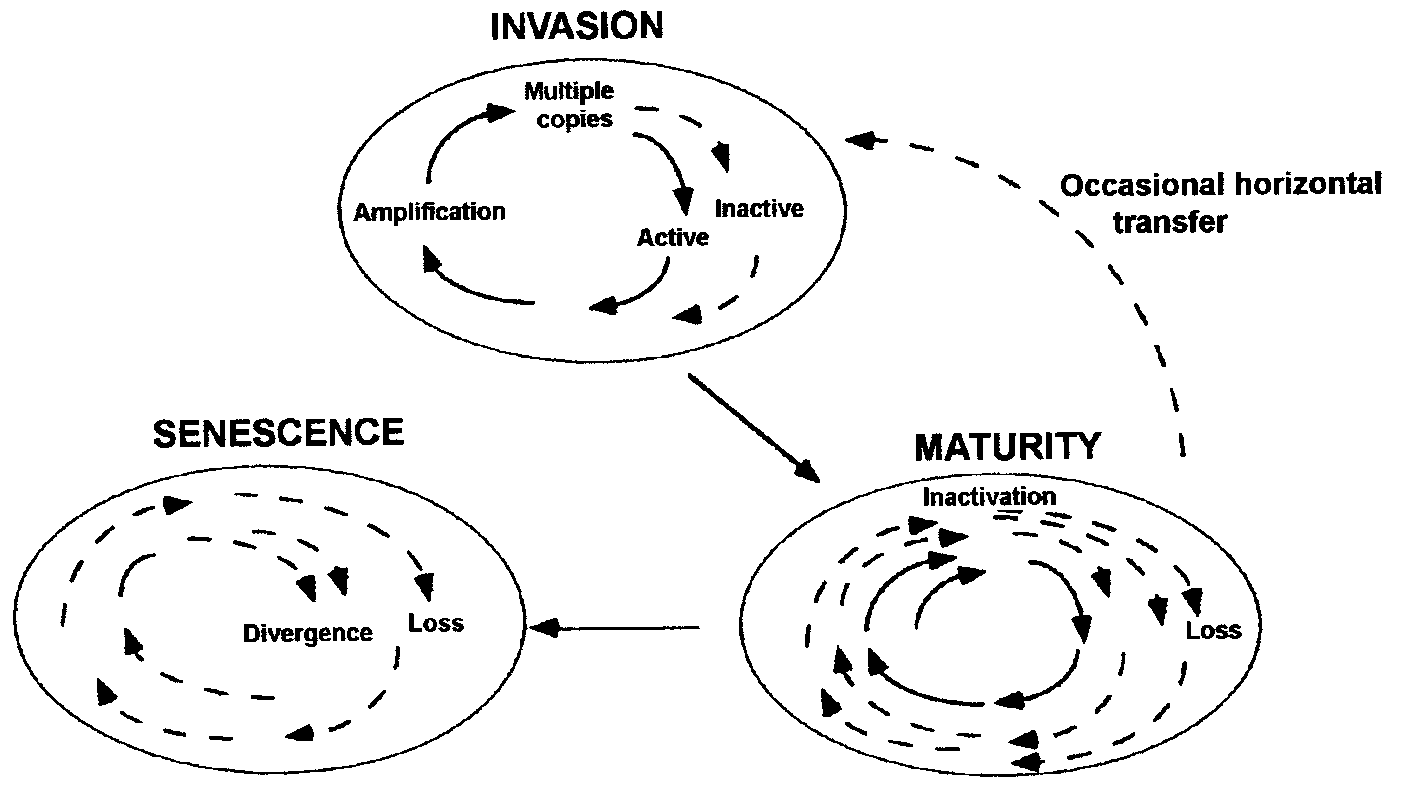
\includegraphics[width=1\textwidth]{figures/cycle.png}
%% \caption{Transposon cycle (\cite{kidwell2001})}
%% \end{figure}

Transposable elements usually undergo some degeneration process, that
inactivates TE copies. We take this phenomenon into account in the
model in the form of an \emph{status score}, that is a fixed number
between zero and one for each TE. When a status of zero is selected,
it renders the TE inactive. This score is also used to determine
whether of not the TE is actively transposing.

Every time a new TE is created from an existing TE, the new copy's
\emph{status score} is chosen to be less than the original score. How
fast this score drops to zero in successive transpositions can be
implemented in several ways, and could be used to reproduce several
interesting scenarios:

\begin{itemize}
\item if the status is constant and zero, then every new copy is
  inactive, and the only active copy is the original one. This is
  known as the \emph{master gene model};

\item if the status is constant and non-zero, then every new copy is
  active, which represents the \emph{transposon model};

\item the status can decrease in a constant rate, which will render
  new copies inactive after a few 

\item the new status can be chosen randomly, between zero and the
  original value
\end{itemize}

\subsubsection{Forms of impact on hosts}

New TEs can cause an impact on the host, depending on where in the
genome it lands when created. This is implemented in the three
categories of insertion sites where TEs might appear. If a TE is
created in a \emph{killer site}, it will be considered a deleterious
transposition. Hosts can be born dead due to deleterious
transposition, and otherwise the impact will be considered a fitness
toll, thus the host will have a lower offspring count when compared.

All transposition models can be used with or without individual
fitness impact on hosts, as an additive fitness impact can be
optionally defined as a config parameter, which is a real number. All
elements that have such an effect on the host are accounted for and
their relative impact is summed and rounded up. This total impact is
the total amount of offspring this particular host will be unable to
produce due to disadvantageous transpositions in its genome.

Lifespan can also be decreased if the impact is too great, albeit not
fatal (as proposed in \cite{rouzic2005}). We include this
characteristic in the model as follows. First we take the ratio
between the total fitness impact as calculated above and the maximum
age defined in the config for the simulation, then this ratio is
rounded down. This integer is the total age classes the host will be
unable to achieve due to deleterious transpositions.


%\subsubsection{Changes in the ammount of copies}

\subsubsection{TE activity dynamics}

Several transposition models can be implemented in the system. We
implemented both neutral models in respect to natural selection
(constant and exponential growth), and a transposition model that
takes into account intrinsic deleterious effects by insertion of new
elements \cite{SKR05}.

Transposition models implemented in our framework have two main
components: one for the the acquisition of new copies and one for the
excision of existing copies.

The acquisition model (usually called by a \verb|transpose()|
function) determines the total amount of new copies that should be
created for the gamete. The excision model (usually called by a
\verb|excise()| function) is the exact opposite. Parameter choices in
the simulation configuration should consider cases where the creation
of new copies never falls behind the deletion of old copies, otherwise
the 

%% Here we describe one of the simplest transposition models we
%% implemented in the simulator. It doesn't take into account any
%% regulation due to selection on the host population, so the only
%% regulation imposed on the TE family, besides self-regulation, is the
%% excision of TE copies. The analytic behaviour of this model is
%% thoroughly described in \cite{rouzic2005}.

%% \begin{equation}
%%   \Delta c_n = (u_n - e) c_n
%% \end{equation}

%% where $c_n$ is the TE count at time $n$, $u_n$ is a decreasing
%% positive function of $n$ and $e>0$. According to this model, the TE
%% can invade the host population provided $u_n$ is larger than $e$ for
%% small $n$ \cite{rouzic2005}, and can fixate if $u_n$ never decreases
%% below $e$. Furthermore, TE copy number reaches an equilibrium if $u_n$
%% converges to $e$ for large $n$.


%% \subsection{The generation algorithm}

%% The general algorithm that happens at each generation models the basic
%% life cycle of a diploid sexual species.

%% \begin{enumerate}
%% \item Host couples are chosen randomly from available mature hosts at
%%   the beginning of each reproductive season. Males are chosen with
%%   replacement, females are chosen without replacement. 

%% \item Each adult bears new gametes after transposition and
%%   recombination.

%% \item Transposition draws a recruitment amount of new TE copies and
%%   the deletion amount of excised copies from the transposition
%%   model. This changes the content of the gametes in terms of
%%   availability of TEs.

%% \item Mutations are sampled from the evolutionary model for newly
%%   created TE copies.

%% \item Recombination provides additional shuffling of gamete contents.

%% \item Each couple gives birth to a number of offspring defined by the
%%   user as a parameter.

%% \item Each newborn individual is composed of one chromosome from each
%%   of its parents, and new individuals are introduced to the population
%%   pool.

%% \item The fitness cost from TEs in newborn individuals is calculated
%%   and any that exceeds a given threshold is killed before birth and
%%   removed from the population. 

%% \item The age of every surviving individuals is incremented ate the
%%   end of the generation.

%% %% \item Newborn individuals inherit one chromosome from each parent,
%% %%   after recombination, transposition and excision of active TEs.

%% \end{enumerate}

% FIXME: diagram in xfig.

\subsection{The population genealogy}
%% Since in the absence of transposition impact the population grows
%% according to the logistic model, we expect $p_n$ not to vary much
%% after a large number of generations, when the parameters are chosen
%% as to minimize phenotypic altering mutations induced by transposition.

We are interested in analyzing sequence data from an individual to
reconstruct the phylogenetic relations between its TEs. Therefore it
becomes necessary to compare the reconstructed history with the real
parental history we simulated.

Each host is identified by a name defined as a serial number, and
carries the names of both parents. A simple recursive breadth-first
algorithm is used to recover the names of parents, grandparents and so
on. As such the genealogy can be fully reconstructed up to any valid
time interval. The population stored in the {\bf Deceased}
compartment can be consulted to create genealogies of different depths
after the execution of the simulation, or inspect each individual for
it's genome, in order to compare the elements present in the sampled
individual, and its ancestors.

\subsection{Sources of stochasticity}
Although most of models described so far involve deterministic models
the overall behavior is stochastic. This happens due to both sampling
effects and the fact that the system is an individual based model, or
agent based model \cite{Bon02}. The following are sources of such
uncertainty:

\begin{enumerate}

\item sampling of individuals in finite population
\label{item:finite}

\item recombination
\label{item:recombination}

\item replication and excision of TEs
\label{item:transposition}

\item mutations (substitutions) within TE sequences
\label{item:mutation}

\end{enumerate}

The item \ref{item:finite} refers to Wright-Fisher models of
populations \cite{HC98}. Since we're simulating small populations
(typically $<10^5$, but there's no restriction to population size)
there is a sampling effect to be considered when an individual is
chosen for reproduction. Should we simulate very large simulations the
importance of sampling effects could be diminished, and we could
approximate the behaviour of an infinite population (as in a
Hardy-Weinberg population).

Since we're simulating sexual populations, we incorporate
recombination by crossing over of games. This can be implemented in
several ways, and the item \ref{item:recombination} is related to the
recombination model used to promote additional variability to the
chromosome pool.

FIXME: falta terminar essa seção.

The item \ref{item:transposition} is related to the availability of
new TEs in the chromosomes (as defined by different \emph{loci} and
sequence).


The item \ref{item:mutation} is related to the evolutionary model used
to promote variability across generations.




\section{Availability}
The simulator has been developed and tested in GNU/Linux systems
running Ubuntu Linux. As it is a portable language, it should run on
any system for which its dependencies are available. Those include Mac
OS X and Windows, besides UNIX/Linux in general. Packaging has been
prepared following guidelines typical of Perl modules and
applications, which should ease the installation in any platform Perl
is available with the help of the CPAN
framework\footnote{http://www.cpan.org}, as well as Debian/Ubuntu DEB
packages.

The software is released in the open-source license GPL and is
available from \url{https://launchpad.net/trepid} .


\section{Implementation details}
\label{sec:implementation}


\subsection{Population models}
\label{sec:impl_pop_models}

\subsubsection{Implementation of the logistic model}

We will use the logistic equation as an example to describe the
implementation because of its simplicity; the implementation of the
Hassel model is analogous.

The differential equation is discretized as a single iteration of
Euler's method, with a step size $h=1$. This results in formula
\eqref{eq:logistic_implem}:

\begin{equation}
  \label{eq:logistic_implem}
  p_{n+1} - p_n = \Delta p = Ceiling \left(  
  \frac{r \times p \times \left(1-\frac{p}{K}\right)}
       {\hbox{offspring count}}  
       \right)
\end{equation}

where $Ceiling(x)$ ($Floor(x)$) is the smallest (greatest) integer
greater (less) than or equal to $x$. Note that this implementation
already takes into account the normalization by the total offspring
count as per equation \eqref{eq:couples}, so the result is the number
of reproducing couples for that generation, instead of the total
income of new individuals.

This model is deterministic so the caching system described in section
\ref{section:impl_caching} is used for it.

\subsubsection{Constant model}

The simplest population model available is arguably the constant
population, which assumes equilibrium and zero net migration. 

The parameter considered for the constant growth is the $r$ config
parameter (reproductive rate), which is used in this case as the total
amount of new individuals to be created for each generation, rounded
up if it's not already an integer.

\begin{equation}
  \Delta p_n = r
\end{equation}


\subsection{Transposition models}
\label{sec:impl_transp_models}
\subsubsection{Exponential model}

The exponential model is a generalization of the constant model, but
instead of only depending on a fixed quantity, it also depends on the
relative number of copies existing at each time. This model also
belongs to a wider class of neutral models that don't take into
account any intrinsic regulation of copy number by fitness
disadvantage to the host \cite{rouzic2005}, where the transposition
rate $u_n$ is a bounded function of $c_n$ and equilibrium is attained
when it saturates at the same value of the excision rate $e$.

\begin{equation}
  \Delta c_n = (u_n - e) c_n
\end{equation}

Considering the transposition rate $u_n$ constant (therefore $u$), it
can be rewritten as:

\begin{equation}
 c_{n+1} - c_n = \Delta c = (u - e) c
\end{equation}

that only depends (deterministically) on the current quantity of
copies $c$ in the reproducing host. As such, the same discretization
scheme used in the population models can be used to provide a
cache-able model that continually increases or decreases copy number
over generations, depending on the value of $u-e$. If $u-e >0$, the
total copy number will always increase, whereas if $u-e<0$ the
simulator will tend to remove more copies that are added.

The model is consulted each time a host produces a gamete both for the
amount of new TE copies to be created, and the amount of existing
copies to be excised. If there must be new TE copies created, for each
new copy a random active TE is sampled (with replacement) from the
host genome, and replicated. Afterwards, if there must be excision of
existing copies, for each excised copy the genome is sampled for a
random TE (without replacement) and this copy is removed from the
genome. Note that only active TEs get transposed, but any TE can be
excised.

\subsubsection{Constant model}

The constant model of transposition is analogous to the respective
population model counterpart. At each time the model is consulted for
the amount of new TE copies to be created, the transposition rate
config parameter $transposition\_rate$ is used as the total amount of
new copies to be generated (rounded up). There is no significant
dynamics in regard to the copy number growth, and it's not bounded per
individual, except for the total number of insertion sites in the
genome, defined in the config file ($killer\_sites$, $severe\_sites$
and $neutral\_sites$). 

The excision of copies is also constant, defined by the config
parameter $e$ as the total amount of previously existing TE copies to
be removed from the gamete.

\begin{equation}
  \Delta c_n = u - e
\end{equation}


\subsubsection{SKR model}

This model assumes an intrinsic self-regulation of TE copy number, and
can assume various shapes and growth forms. The original article
proposes that the form of the $U(c_n)$ function can be chosen as any
functions that share the qualitative behaviour described, and suggests
(and tests) three forms indexed as $U_1$, $U_2$ and $U_3$ that we
reproduced in this framework.

\begin{equation}
  c_{n+1} = Ceiling(c_n + c_n \times T_0 \times U (c_n ))
\end{equation}

\begin{equation}
  U_1(c) = 2^{(-c/C_{0.5})}
\end{equation}

\begin{equation}
  U_2 (c) = 1 - \frac{c^5} {(C_{0.5}^5 + c^5 )}
\end{equation}

\begin{equation}
  U_3 (c) = 1 + (c - \frac{0.5}{C_{0.5}} )
\end{equation}

Transposition with this model is provided by the preceding equations,
while excision is provided by the exact same function of the
exponential model.

\subsection{Caching of deterministic models}
\label{section:impl_caching}

In order to save unnecessary calculations, caching of model data is
implemented for both population and transposition models. All values
calculated for deterministic models are cached to avoid the
performance toll of unnecessary repeated calculations. This cache is
implemented as a hash\footnote{Sometimes referred to as an associative
  array.}, and is consulted before each calculation to see if it's
necessary.

The cached data are stored independently per simulation and per data
type (population or transposition), so in case a user wants to
instantiate several different simulations in the same
session \footnote{This functionally requires usage of the library via
  the API. A sample script is provided as an example for
  programmers.}, data from different simulations are guaranteed not to
mix.


\section{Data structures}
The model is implemented in Perl5, using its object-oriented
paradigm. The main classes \verb|TRepid::Population|,
\verb|TRepid::Host| and \verb|TRepid::TE| define, respectively,
objects for the population, the hosts that constitute the population
and the TEs that populate each host genome.

Two classes inherit methods from Bioperl classes \cite{SBB+02}. The TE
class inherits the \verb|Bio::Seq| class, and the Host class inherits
the \verb|Bio::SeqIO| class. This guarantees the simulator can import
and export sequences using a great range of sequence formats. It also
uses the abstract model of representing DNA sequences provided by the
Bioperl project in a way that unifies the usage of any sequence format
(Fasta, genbank, embl, swissprot, etc) so that any of these formats
can be used at the discretion of the user. We provide a wrapper for
including header information in the Fasta format, which we describe in
detail in a later section.

The documentation of the API is bundled within the code with the POD
(Plain Old Documentation) format, which can be accessed by the
ordinary means of any Perl distribution. Besides being available
inline in the code, all this material is also converted and provided
in more convenient formats like HTML and PDF.

\subsection{Host data structure}
The structure inherited from \verb|Bio::SeqIO| provide methods to
collect and save sequences from a file, which inspired an
implementation for a file-based storage. Besides these
general-purposed methods we defined some object attributes to store
meta-data related to each individual like its name, age, gender,
fitness, the two chromosomes the file name to which the \verb|Host|
object is associated.

Each of the two chromosomes is an array, and each of its positions
stores a reference for a TE object if one is present. Methods for
consulting the number or position of TEs and de-reference them are
provided in the class API.

\subsection{Population data structure}
The object attributes for the \verb|Population| class store
information related to where the files are stored in disk, and some
statistics that are frequently consulted.

%% The population is stored in a hash with the host name as hash key and
%% the reference to the \verb|Host| object as the hash value. The
%% reference to this hash is stored in a scalar object attribute
%% \verb|POP|.

\subsection{TE data structure}

Besides the structure inherited from \verb|Bio::Seq|, which includes
methods for setting and retrieving several meta-data as the sequence
string, header information, etc.



\subsection{Meta-data format for Fasta sequences}

We default to using sequences in Fasta format. To this end, we propose
a protocol for inserting meta-data into the Fasta header and a set of
corresponding parser (writer) methods in order to retrieve (save) the
corresponding information.

%% This is the template for a typical Fasta header as used in the TRepid
%% simulator. The fields are separated by colons (:), and the following template
%% shows the type of variable to be expected in each field.

\bigskip
\verb|>string:int:int:real|
\bigskip

The first field (string) denotes the {\bf TE description}. It can vary
in size and can contain spaces. Usually it comprises the whole Fasta
header if a real sequence is used, as acquired from any genomic
database, should one such sequence be used.

The next two fields that contain integer numbers. The first is the
{\bf site} position in the chromosome, and the second defines in which
{\bf chromosome} this particular TE is located. The total number of
sites available can be chosen by the user, and the default is 100
positions (from 0 to 99). There are always two chromosomes (denoted by
the numbers 0 and 1) since we are modelling sexual diploid
populations.

The last field is a real number, in the interval $[0,1]$. It describes
the {\bf status score} of activity for that TE, where any non-zero
value means the TE is active. Each new copy generated from this copy
should have a lower score, effectively reproducing a deactivation
function for the TE family.


%% - Field Fitness (real)
%% Characterizes the strain transmissibility, in the probability of it
%% being transfered.
%% Can assume values in the [0,1] interval.
%% A value of 0 means the strain is inactive.

%% The basic FASTA header is incremented with model information from
%% several coded fields, separated by colon (:).



%%%%%%%%%%%%%%%%%%%%%%%%%%%%%%%%
%% \section{Authors contributions}
%%     Text for this section \ldots



%% FIXME: incluir discussões sobre:

%% - Gene drive system x mechanism (James 2005, Sinkins 2006) \cite{james2005,SG06}

%% - wright-fisher models (livro hartl)\cite{HC98}

%% - finite population

%% - infinite-sites model, infinite-allelles model \cite{Taj96}

%% - forward-time simulator (paper SFS, papers afins)

%% - agent-based model \cite{Bon02}

%% - phylodynamics (paper volz, papers claudio) \cite{VKP+09,SMT+09}




\bibliographystyle{natbib}  % Style BST file
\bibliography{ffigueiredo-cjs_trepid_bibtex}      % Bibliography file (usually '*.bib' )
%% }

%%%%%%%%%%%



%% \appendix
%% \section{API description}

%% The following sections document the API of the simulator, which is
%% available for scripting arbitrary simulations in the Perl
%% language. The main classes are described here in this document, and
%% the classes of  \ldots

%% \section{TRepid}
%% \subsection{NAME\label{NAME}\index{NAME}}


TRepid

\subsection{DESCRIPTION\label{DESCRIPTION}\index{DESCRIPTION}}


Main class for simulation of Transposon evolution

\subsubsection*{Primary functions\label{Primary_functions}\index{Primary functions}}
\paragraph*{prepare()\label{prepare_}\index{prepare()}}


This function will load a previously existing population from disk, if
one exists, or initialize a new population of otherwise. It will also
make sure all required options are collected from trepid.conf, or that
defaults are in usad.

\paragraph*{simulate()\label{simulate_}\index{simulate()}}


This function runs a simulation, consisting of several generations of
the Host population, cf. defined in trepid.conf

\paragraph*{save()\label{save_}\index{save()}}


This function saves the population from memory to disk.

\paragraph*{clean()\label{clean_}\index{clean()}}


This function erases the population from memory.

\paragraph*{run()\label{run_}\index{run()}}


This is just a quick way to run automatically. It calls prepare(), then
simulate().

\subsubsection*{Secondary functions\label{Secondary_functions}\index{Secondary functions}}
\paragraph*{non\_interactive\_preload()\label{non_interactive_preload_}\index{non\ interactive\ preload()}}


This function does the initial configuring before saving options are
parsed. This includes printing a header for the simulation and making
sure the data directories are present and accessible.

\paragraph*{interactive\_preload()\label{interactive_preload_}\index{interactive\ preload()}}


This function asks questions on what to save after the simulation, if
interactiveness is permitted. A non-interactive simulation will occur
if any of the following occur:



- all options are explicitly specified in trepid.conf
- the "interactive" option is set to 0 in trepid.conf

\paragraph*{save\_check()\label{save_check_}\index{save\ check()}}


This function parses variables that are collected either from
interactive\_preload or trepid.conf, and make sure they're usable.



%% \section{TRepid::Host}
%% \subsection{NAME\label{NAME}\index{NAME}}


TRepid::Host

\subsection{DESCRIPTION\label{DESCRIPTION}\index{DESCRIPTION}}


Hosts class for TRepid.

\subsubsection*{OBJECT ATTRIBUTES\label{OBJECT_ATTRIBUTES}\index{OBJECT ATTRIBUTES}}


Atributes

\paragraph*{NAME\label{NAME}\index{NAME}}


Is a string, and it should be unique in the population. If the user
lets the names be auto-generated, they will be sequential integers.

\paragraph*{GENDER\label{GENDER}\index{GENDER}}


Is a single character: M for Male and F for female.

\paragraph*{FITNESS\label{FITNESS}\index{FITNESS}}


The total count of offspring this host generated so far.

\paragraph*{AGE\label{AGE}\index{AGE}}


Is an integer. Offspring are auto-generated with age 0 (as oposed to
1), and it can be increased until it reaches \$age\_max (which is set in
TRepid::Conf

\paragraph*{GM\label{GM}\index{GM}}


Is an integer. Represents the total TE count in the host's genome.

\paragraph*{STRAND1\label{STRAND1}\index{STRAND1}}


The list of insertion sites. Is a reference to an array of TRepid::TE
objects, or undef values. Strand1 is the dna strand originated from

\paragraph*{STRAND2\label{STRAND2}\index{STRAND2}}


See STRAND1

\paragraph*{FILE\label{FILE}\index{FILE}}


The original file name, if this individual existed on disk previous to
simulation start. In this case, the host's attributes are loaded from
the file (relative path).

\paragraph*{NEWFILE\label{NEWFILE}\index{NEWFILE}}


The name the file will have when it's saved. The filename will be
updated at the end of the simulation to reflect any changes in the
attributes (like age, for example).

\subsection{METHODS\label{METHODS}\index{METHODS}}


The following methods are available from this class. Internal methods
are usually preceded with a \_

\subsubsection*{Basic Methods\label{Basic_Methods}\index{Basic Methods}}
\paragraph*{new\label{new}\index{new}}
\begin{verbatim}
 Title   : new
 Usage   :
 Function: 
 Example :
 Returns :
 Args    :
 Requires: FILE || NAME, GENDER, FITNESS, AGE, PARENTS, STRAND1, STRAND2
\end{verbatim}
\paragraph*{file\label{file}\index{file}}
\begin{verbatim}
 Title   : file
 Usage   : $filename = $host->file;
           file('adam-M-50-2');
\end{verbatim}
\begin{verbatim}
 Function: Returns the filename if called without arguments
           Sets filename if called with argument
\end{verbatim}
\begin{verbatim}
 Example :
 Returns : string
 Args    : [optional] filename
 Requires:
\end{verbatim}
\paragraph*{name\label{name}\index{name}}
\begin{verbatim}
 Title   : name
\end{verbatim}
\begin{verbatim}
 Usage   : $name = name();
           name('adam');
\end{verbatim}
\begin{verbatim}
 Function: Returns the host name if called without arguments
           Sets host name if called with argument
\end{verbatim}
\begin{verbatim}
 Example :
 Returns : string
 Args    : [optional] string
 Requires:
\end{verbatim}
\paragraph*{gender\label{gender}\index{gender}}
\begin{verbatim}
 Title   : gender
\end{verbatim}
\begin{verbatim}
 Usage   : $gender = gender();
           gender('M');
\end{verbatim}
\begin{verbatim}
 Function: Returns the host gender if called without arguments
           Sets host gender if called with argument
\end{verbatim}
\begin{verbatim}
 Example :
 Returns :
 Args    :
 Requires:
\end{verbatim}


Gender can be one of 'M' or 'F'.

\paragraph*{age\label{age}\index{age}}


Title   : age



Usage   : \$age = age();
          age(2);



Function: 
Example :
Returns : integer
Args    : [optional] integer
 Requires:

\paragraph*{fitness\label{fitness}\index{fitness}}
\begin{verbatim}
 Title   : fitness
 Usage   : $fitness = fitness()
          fitness(50)
\end{verbatim}
\begin{verbatim}
 Function: 
 Example :
 Returns : integer
 Args    : [optional] integer
 Requires:
\end{verbatim}


The number of offpsring this ::Host has generated so far. It will be
updated by Population::offspring()

\paragraph*{strand1\label{strand1}\index{strand1}}
\begin{verbatim}
 Title   : strand1
 Usage   :
 Function: 
 Example :
 Returns : 
 Args    : [optional] DNA strand
 Requires:
\end{verbatim}
\paragraph*{strand2\label{strand2}\index{strand2}}
\begin{verbatim}
 Title   : strand2
 Usage   : 
 Function: 
 Example : 
 Returns : 
 Args    : [optional] DNA strand
 Requires:
\end{verbatim}
\paragraph*{heritage\label{heritage}\index{heritage}}
\begin{verbatim}
 Title   : heritage
 Usage   :
 Function: Defines the genetic heritage of the offspring
 Example :
 Returns : DNA strand
 Args    : [optional] two refs to DNA strands
 Requires: STRAND1, STRAND2
\end{verbatim}


The heritage() method randomly selects one DNA strand from each parent
and injects one strand from each parent into the offspring as his own
strands. Offspring's strand 1 comes from male parent, and strand 2
comes from female parent.



Each strand is a reference to an array of Bio::Seq objects, in no
particular order.

\paragraph*{recombine\label{recombine}\index{recombine}}
\begin{verbatim}
 Title   : recombine
 Usage   : 
 Function: Recombination of 
 Example : 
 Returns : DNA strand
 Args    : [optional] two refs to DNA strands
 Requires: STRAND1, STRAND2
\end{verbatim}


The recombine() method returns a gamete after a 'crossing over'
process. The gamete is just a STRAND.



The particular method of recombining is choosen in the trepid.conf
file, with the recombination\_model variable.

\paragraph*{recombine\_allstep\label{recombine_allstep}\index{recombine\ allstep}}
\begin{verbatim}
 Title   : recombine_allstep
 Usage   : 
 Function: Recombination of 
 Example : 
 Returns : DNA strand
 Args    : [optional] two refs to DNA strands
 Requires: STRAND1, STRAND2
\end{verbatim}


The recombine() method returns a gamete after a 'crossing over'
process. The gamete is just a STRAND.

\paragraph*{recombine\_2step\label{recombine_2step}\index{recombine\ 2step}}
\begin{verbatim}
 Title   : recombine_2step
 Usage   : 
 Function: Recombination of 
 Example : 
 Returns : DNA strand
 Args    : [optional] two refs to DNA strands
 Requires: STRAND1, STRAND2
\end{verbatim}


The recombine() method returns a gamete after a 'crossing over'
process. The gamete is just a STRAND.



Chooses two insertion sites and swap the strands' sites between the two sites.

\paragraph*{recombine\_1step\label{recombine_1step}\index{recombine\ 1step}}
\begin{verbatim}
 Title   : recombine_1step
 Usage   : 
 Function: Recombination of 
 Example : 
 Returns : DNA strand
 Args    : [optional] two refs to DNA strands
 Requires: STRAND1, STRAND2
\end{verbatim}


The recombine() method returns a gamete after a 'crossing over'
process. The gamete is just a STRAND.



Chooses one insertion sites and swap the strands' sites after that site.

\paragraph*{recombine\_none\label{recombine_none}\index{recombine\ none}}
\begin{verbatim}
 Title   : recombine_none
 Usage   : 
 Function: 
 Example : 
 Returns : DNA strand
 Args    : [optional] two refs to DNA strands
 Requires: STRAND1, STRAND2
\end{verbatim}


The recombine() method returns a gamete after a 'crossing over'
process. The gamete is just a STRAND.



This trivial recombination model does not recombine with crossover,
and just returns one of the two strands at random.

\paragraph*{TE\_excise\label{TE_excise}\index{TE\ excise}}
\begin{verbatim}
 Title   : TE_excise
 Usage   :
 Function: Excise a TE from the Host's genome
 Example :
 Returns : Boolean
 Args    : extended site
 Requires: STRAND1, STRAND2
\end{verbatim}
\paragraph*{TE\_random\label{TE_random}\index{TE\ random}}
\begin{verbatim}
 Title   : TE_random
 Usage   : 
 Function: Select a random TE
 Example : 
 Returns : TRepid::TE object
 Args    : 
 Requires: STRAND1, STRAND2
\end{verbatim}


Selects a random TE from either STRAND1 or STRAND2. If there are no
TEs, returns false.

\paragraph*{TE\_by\_extended\_site\label{TE_by_extended_site}\index{TE\ by\ extended\ site}}
\begin{verbatim}
 Title   : TE_by_extended_site
 Usage   : 
 Function: Return a TE given its extended site
 Example : 
 Returns : TRepid::TE object
 Args    : Extended site
 Requires: STRAND1, STRAND2
\end{verbatim}
\paragraph*{TE\_active\label{TE_active}\index{TE\ active}}
\begin{verbatim}
 Title   : TE_active
 Usage   : 
 Function: Select a random active TE
 Example : 
 Returns : TRepid::TE object
 Args    : 
 Requires: STRAND1, STRAND2
\end{verbatim}


Selects a random active TE from either STRAND1 or STRAND2

\paragraph*{TE\_find\label{TE_find}\index{TE\ find}}
\begin{verbatim}
 Title   : TE_find
 Usage   : $host->TE_find('transposon123')
           $host->TE_find('^gypsy.*')
 Function: Search TE by name (perl regexp).
 Example : 
 Returns : list of extended sites
 Args    : string to match TE name
 Requires: STRAND1, STRAND2
\end{verbatim}


Case sensitive. See perldoc perlre and perldoc perlretut for more
information on perl regexps.

\paragraph*{TE\_sites\_list\label{TE_sites_list}\index{TE\ sites\ list}}
\begin{verbatim}
 Title   : TE_sites_list
 Usage   :
 Function: Return list of list of extended sites
 Example :
 Returns : array
 Args    : [optional]  two refs to DNA strands
 Requires: STRAND1, STRAND2
\end{verbatim}
\paragraph*{TE\_active\_list\label{TE_active_list}\index{TE\ active\ list}}
\begin{verbatim}
 Title   : TE_active_list
 Usage   : 
 Function: Returns the list of active TEs' extended sites 
 Example : 
 Returns : array
 Args    : 
 Requires: STRAND1, STRAND2
\end{verbatim}
\paragraph*{parents\label{parents}\index{parents}}
\begin{verbatim}
 Title   : parents
 Usage   : parents()
           parents(["adam", "eve"])
 Function: Returns the filename if called without arguments
           Sets filename if called with argument
\end{verbatim}
\begin{verbatim}
 Example :
 Returns : arrayref to (father, mother) names
 Args    : [optional] arrayref to (father, mother) names
 Requires: PARENTS
\end{verbatim}
\paragraph*{newfile\label{newfile}\index{newfile}}
\begin{verbatim}
 Title   : newfile
 Usage   : $newfile = newfile();
           newfile('adam-M-50-4')
\end{verbatim}
\begin{verbatim}
 Function: 
 Example :
 Returns :
 Args    :
 Requires:
\end{verbatim}
\paragraph*{is\_wild\label{is_wild}\index{is\ wild}}
\begin{verbatim}
 Title   : is_wild
 Usage   :
 Function: 
 Example :
 Returns : Boolean
 Args    :
 Requires:
\end{verbatim}
\paragraph*{is\_gm\label{is_gm}\index{is\ gm}}
\begin{verbatim}
 Title   : is_gm
 Usage   :
\end{verbatim}
\begin{verbatim}
 Function: Returns te TE count (non-zero is GM, zero is wild)
           Sets death by excessive TE count
\end{verbatim}
\begin{verbatim}
 Example :
 Returns : integer
 Args    : [optional] integer
 Requires:
\end{verbatim}


Note: is\_gm() does only return the TE count, NOT update it.

\paragraph*{is\_dead\label{is_dead}\index{is\ dead}}
\begin{verbatim}
 Title   : is_dead
 Usage   :
 Function: Returns/sets the dead value (non-zero is dead)
 Example :
 Returns : Boolean
 Args    : [optional] Boolean
 Requires:
\end{verbatim}
\paragraph*{is\_mature\label{is_mature}\index{is\ mature}}
\begin{verbatim}
 Title   : is_mature
 Usage   :
 Function: 
 Example :
 Returns : Boolean
 Args    :
 Requires:
\end{verbatim}
\paragraph*{age\_increment\label{age_increment}\index{age\ increment}}
\begin{verbatim}
 Title   : age_increment
 Usage   :
 Function: 
 Example :
 Returns :
 Args    :
 Requires:
\end{verbatim}


Increments age. Also updates the DEAD property, i.e., sets death by age, or transposition impact if necessary.

\paragraph*{syncFS\label{syncFS}\index{syncFS}}
\begin{verbatim}
 Title   : syncFS
 Usage   : $host->syncFS
           $host->syncFS($file)
\end{verbatim}
\begin{verbatim}
 Function: 
 Example : 
 Returns : NEWFILE (or FILE)
 Args    : [optional] file name
 Requires: NEWFILE (or FILE)
\end{verbatim}


The \_newfile() update (or newfile() directly) should be done
previously to saving the object to disk. Normally, this is handled by
Population::syncFS().



If called with a parameter, it gets assigned to NEWFILE, which is the
preferred filename to be used.

\paragraph*{\_newfile\label{_newfile}\index{\ newfile}}
\begin{verbatim}
 Title   : _newfile
 Usage   : Updates the NEWFILE attribute
 Function: 
 Example : 
 Returns : string (NEWFILE)
 Args    : 
 Requires: NAME, AGE, GENDER, FITNESS, PARENTS
\end{verbatim}


Updates the NEWFILE attribute according to current attributes. For the
accessor method, see the "newfile()" method.

\paragraph*{\_write\_seqs\_fasta\label{_write_seqs_fasta}\index{\ write\ seqs\ fasta}}
\begin{verbatim}
 Title   : _write_seqs_fasta
 Usage   : 
 Function: 
 Example : 
 Returns : string (filename)
 Args    : 
 Requires: NEWFILE||FILE, STRAND1, STRAND2
\end{verbatim}
\paragraph*{show\label{show}\index{show}}
\begin{verbatim}
 Title   : show
 Usage   : 
 Function: 
 Example : 
 Returns : string
 Args    : 
 Requires: NAME, GENDER, AGE, FITNESS, GM, NEWFILE||FILE
\end{verbatim}


This method does not require the host to be alive, so should not be
used to print individual information of whole populations. For that,
use the table\_show() method below.

\paragraph*{table\_show\label{table_show}\index{table\ show}}
\begin{verbatim}
 Title   : table_show
 Usage   : 
 Function: 
 Example : 
 Returns : string
 Args    : 
 Requires: DEAD=0, NAME, GENDER, AGE, FITNESS, GM, NEWFILE||FILE
\end{verbatim}


The table\_show() method is used to print summarized information of
individual hosts. See also TRepid::Population::show().

\paragraph*{TE\_show\label{TE_show}\index{TE\ show}}
\begin{verbatim}
 Title   : TE_show
 Usage   :
 Function: 
 Example :
 Returns : string
 Args    :
 Requires:
\end{verbatim}
\paragraph*{fitness\_impact\label{fitness_impact}\index{fitness\ impact}}
\begin{verbatim}
 Title   : fitness_impact
 Usage   : $lost_offspring = $h->fitness_impact
 Function: 
 Example : 
 Returns : integer
 Args    :
 Requires:
\end{verbatim}


Returns the mean cost of fitness before mating. The fitness cost is given as the ammount of offpsring not created when this host mates due to transposition effects.



This does not take into account offspring that are born dead because of deleterious transposition.



%% \section{TRepid::Population}
%% \subsection{NAME\label{NAME}\index{NAME}}


TRepid::Population

\subsection{DESCRIPTION\label{DESCRIPTION}\index{DESCRIPTION}}


Population class for TRepid

\subsubsection*{OBJECT ATTRIBUTES\label{OBJECT_ATTRIBUTES}\index{OBJECT ATTRIBUTES}}
\paragraph*{DATADIR\label{DATADIR}\index{DATADIR}}


The directory where the population is stored on disk.

\paragraph*{POP\label{POP}\index{POP}}


Hash reference of TRepid::Host indexed by Host name.

\paragraph*{DEAD\label{DEAD}\index{DEAD}}


see POP

\paragraph*{SIZE\label{SIZE}\index{SIZE}}


The size of the population.

\paragraph*{TE\label{TE}\index{TE}}


How many TEs (total) there are in the population.

\paragraph*{FITNESS\label{FITNESS}\index{FITNESS}}


The mean fitness of the population

\paragraph*{LOG\label{LOG}\index{LOG}}


Contatenation of strings (log messages), that can be saved to logfile.

\subsection{METHODS\label{METHODS}\index{METHODS}}
\subsubsection*{Methods for population management\label{Methods_for_population_management}\index{Methods for population management}}


The following methods are available from this class.



Internal methods are usually preceded with a \_

\paragraph*{new\label{new}\index{new}}
\begin{verbatim}
 Title   : new
 Usage   : $pop->new(DATADIR=>"data")
 Function: Creates a new population
 Example :
 Returns :
 Args    : 
 Requires: DATADIR or ($data_dir in TRepid::Conf)
\end{verbatim}


The new() method initializes an empty population object, ready to be
created (with init()) or loaded from disk (with collect()).

\paragraph*{collect\label{collect}\index{collect}}
\begin{verbatim}
 Title   : collect
 Usage   : $pop->collect
 Function: Loads existing population from disk into memory
 Example :
 Returns : POP
 Args    : none
 Requires: DATADIR
\end{verbatim}


The collect() method will create one TRepid::Host object per file
found in the DATADIR directory, which is assumed to be set, and
exist. Each filename will be automatically parsed by the proper method
in the Hosts class.

\paragraph*{collect\_fast\label{collect_fast}\index{collect\ fast}}
\begin{verbatim}
 Title   : collect_fast
 Usage   : $pop->collect_fast
 Function: Loads existing population from disk into memory
 Example :
 Returns : POP
 Args    : 
 Requires: DATADIR
\end{verbatim}


Same as collect() method, but only parses Wild and GM directories (not
Deceased)

\paragraph*{init\label{init}\index{init}}
\begin{verbatim}
 Title   : init
 Usage   : $pop->init
 Function: Inits a new population in the disk
 Example :
 Returns : POP
 Args    : 
 Requires: DATADIR
\end{verbatim}
\paragraph*{clear\label{clear}\index{clear}}
\begin{verbatim}
 Title   : clear
 Usage   : $pop->clear
 Function: Clears the whole population from memory
 Example :
 Returns :
 Args    : 
 Requires: POP, DEAD
\end{verbatim}


Deletes the references for all TRepid::Host objects, forcing perl to
clear them from memory.

\paragraph*{wipe\label{wipe}\index{wipe}}
\begin{verbatim}
 Title   : wipe
 Usage   : &TRepid::Population::wipe
 Function: Fast way to clean the whole population on disk
 Example :
 Returns :
 Args    : 
 Requires:
\end{verbatim}


Fast-deletes all files in the compartment sub-directories of DATADIR.



Obs: this is a function, not a method!

\paragraph*{pop\label{pop}\index{pop}}
\begin{verbatim}
 Title   : pop
 Usage   : $ref = $population->pop
 Function: Returns the live population 
 Example :
 Returns : Reference of a hash of TRepid::Host objects
 Args    :
 Requires: POP
\end{verbatim}


The hash is indexed by the host's name, i.e., (key,value)=(name,obj).

\paragraph*{dead\label{dead}\index{dead}}
\begin{verbatim}
 Title   : dead
 Usage   : @dead = $pop->dead
 Function: Returns the dead population
 Example :
 Returns : Reference of a hash of TRepid::Host objects
 Args    :
 Requires: DEAD
\end{verbatim}


The hash is indexed by the host's name, i.e., (key,value)=(name,obj).

\paragraph*{couple\label{couple}\index{couple}}
\begin{verbatim}
 Title   : couple
 Usage   : @couple = $pop->couple
 Function: Choose Male and Female, and copulate them
 Example :
 Returns :
 Args    : list of TRepid::Host names
 Requires: POP
\end{verbatim}


Choose a random mating pair in the population, suitable for input to
offpsring().

\paragraph*{offspring\label{offspring}\index{offspring}}
\begin{verbatim}
 Title   : offspring
 Usage   : $child = $pop->offspring(@couple)
 Function: Copulate Male and Female and generate one offspring
 Example : $child = $pop->offspring("adam", "eve", "caim")
 Returns : new TRepid::Host object
\end{verbatim}
\begin{verbatim}
 Args    : two string parameters (male and female parents names)
           [optional] third argument (offspring's name)
\end{verbatim}
\begin{verbatim}
 Requires: POP
\end{verbatim}


The iteration needed for multiple offsprings is not done by this method.

\paragraph*{sample\label{sample}\index{sample}}
\begin{verbatim}
 Title   : sample
 Usage   : $host = $pop->sample
 Function: Samples the population for a random host
 Example : $gm_host = $pop->sample( $pop->gm )
 Returns : string (TRepid::Host name)
 Args    : [optional] list of TRepid::Host names
 Requires: POP
\end{verbatim}
\paragraph*{syncFS\label{syncFS}\index{syncFS}}
\begin{verbatim}
 Title   : syncFS
 Usage   : $pop->syncFS
 Function: Saves changes to Hosts' files on disk
 Example :
 Returns :
 Args    :
 Requires: POP, DEAD
\end{verbatim}


The syncFS() method uses the TRepid::Host::syncFS() method to save each
host into its new filename.

\paragraph*{host\label{host}\index{host}}
\begin{verbatim}
 Title   : host
 Usage   : $host = $pop->host("adam")
 Function: Return TRepid::Host object, by name
 Example : 
 Returns : TRepid::Host object
 Args    : string (name)
 Requires: POP
\end{verbatim}


Easy method to retrieve a host by its name.

\subsubsection*{Methods that return list of names satisfying attribute choice\label{Methods_that_return_list_of_names_satisfying_attribute_choice}\index{Methods that return list of names satisfying attribute choice}}
\paragraph*{wild\label{wild}\index{wild}}
\begin{verbatim}
 Title   : wild
 Usage   : @names = $pop->wild
 Function: 
 Example :
 Returns : List of TRepid::Host names
 Args    : 
 Requires: POP
\end{verbatim}
\paragraph*{gm\label{gm}\index{gm}}
\begin{verbatim}
 Title   : gm
 Usage   : @names = $pop->gm
 Function: 
 Example : 
 Returns : List of TRepid::Host names
 Args    : 
 Requires: POP
\end{verbatim}
\paragraph*{are\_dead\label{are_dead}\index{are\ dead}}
\begin{verbatim}
 Title   : are_dead
 Usage   : @names = $pop->are_dead
 Function: 
 Example : 
 Returns : List of TRepid::Host names
 Args    : 
 Requires: DEAD
\end{verbatim}


Cemetery. See the \_dead() method to update the list, prior to returning it.

\paragraph*{not\_dead\label{not_dead}\index{not\ dead}}
\begin{verbatim}
 Title   : not_dead
 Usage   : @names = $pop->not_dead
 Function: 
 Example : 
 Returns : List of TRepid::Host names
 Args    : 
 Requires: POP
\end{verbatim}


not\_dead() returns a list of names, while size() returns an integer.

\paragraph*{males\label{males}\index{males}}
\begin{verbatim}
 Title   : males
 Usage   : @names = $pop->males
 Function: 
 Example : 
 Returns : list of names
 Args    : 
 Requires:
\end{verbatim}
\paragraph*{females\label{females}\index{females}}
\begin{verbatim}
 Title   : females
 Usage   : @names = $pop->females
 Function: 
 Example : 
 Returns : list of names
 Args    : 
 Requires:
\end{verbatim}
\paragraph*{mature\label{mature}\index{mature}}
\begin{verbatim}
 Title   : mature
 Usage   : @names = $pop->mature
 Function: Returns list of names of sexually mature TRepid::Host
 Example :
 Returns : integer
 Args    :
 Requires: POP
\end{verbatim}
\paragraph*{are\_gender\label{are_gender}\index{are\ gender}}
\begin{verbatim}
 Title   : are_gender
 Usage   : @names = $pop->are_gender
 Function: 
 Example : 
 Returns : list of strings
 Args    : [optional] list of names
 Requires: POP
\end{verbatim}
\paragraph*{TE\_find\label{TE_find}\index{TE\ find}}
\begin{verbatim}
 Title   : TE_find
 Usage   : @names = $pop->TE_find("te_family1")
 Function: 
 Example : 
 Returns : list of strings
 Args    : string to match TE name
 Requires: POP
\end{verbatim}
\subsubsection*{Methods for data collection and Statistics\label{Methods_for_data_collection_and_Statistics}\index{Methods for data collection and Statistics}}
\paragraph*{size\label{size}\index{size}}
\begin{verbatim}
 Title   : size
 Usage   : $size = $pop->size
 Function: Returns the population size
 Example :
 Returns : integer
 Args    :
 Requires: POP
\end{verbatim}


The size() method only accesses the SIZE attribute. To actually update
the population size, use the \_size() method.

\paragraph*{TE\_total\label{TE_total}\index{TE\ total}}
\begin{verbatim}
 Title   : TE_total
 Usage   : $Total_TEs $pop->TE_total
 Function: 
 Example : 
 Returns : integer
 Args    : 
 Requires:
\end{verbatim}
\paragraph*{TE\_mean\label{TE_mean}\index{TE\ mean}}
\begin{verbatim}
 Title   : TE_mean
 Usage   : 
 Function: 
 Example : 
 Returns : real
 Args    : 
 Requires:
\end{verbatim}
\paragraph*{TE\_total\_active\label{TE_total_active}\index{TE\ total\ active}}
\begin{verbatim}
 Title   : TE_total_active
 Usage   : 
 Function: 
 Example : 
 Returns : integer
 Args    : 
 Requires:
\end{verbatim}
\subsubsection*{Methods for results management\label{Methods_for_results_management}\index{Methods for results management}}
\paragraph*{show\label{show}\index{show}}
\begin{verbatim}
 Title   : show
 Usage   : print $pop->show
 Function: Returns printable string for population display.
 Example :
 Returns : Formatted printable string of population for screen display.
 Args    :
 Requires: POP
\end{verbatim}


The show() method returns a printable string of TAB separated values
format of each host currently alive in the population.



* WARNING * Beware of show() on large populations - each individual
  will take one line of screen, and with several thousands of
  individuals it may not be what you want.

\paragraph*{show\_summary\label{show_summary}\index{show\ summary}}
\begin{verbatim}
 Title   : show_summary
 Usage   : print $pop->show
 Function: Returns printable selected config parameters.
 Example : 
 Returns : Formatted printable string with population summary information
 Args    : 
 Requires: POP, DEAD
\end{verbatim}
\paragraph*{log\label{log}\index{log}}
\begin{verbatim}
 Title   : log
 Usage   : $pop->log("message")
 Function: update log queue on RAM and prints message to screen
 Example : 
 Returns : 
 Args    : string (log message)
 Requires:
\end{verbatim}


The log() method updates the log queue on memory. To save it do disk, use
the synclog() method.

\paragraph*{synclog\label{synclog}\index{synclog}}
\begin{verbatim}
 Title   : synclog
 Usage   : $pop->synclog
 Function: 
 Example : 
 Returns : 
 Args    : 
 Requires: LOG
\end{verbatim}


The synclog() method saves the log queue to disk in the file define in
the \$log\_file var.

\subsubsection*{Methods that update population attributes\label{Methods_that_update_population_attributes}\index{Methods that update population attributes}}
\paragraph*{fitness\label{fitness}\index{fitness}}
\begin{verbatim}
 Title   : fitness
 Usage   :
 Function: Returns the population fitness
 Example :
 Returns : real
 Args    : [optional] list of TRepid::Host names
 Requires: [optional] POP
\end{verbatim}


The population fitness is defined here as the arithmetic mean of the
hosts' fitnesses (average offspring number).

\paragraph*{\_TE\_total\label{_TE_total}\index{\ TE\ total}}
\begin{verbatim}
 Title   : _TE_total
 Usage   : 
 Function: 
 Example : 
 Returns : integer
 Args    : 
 Requires:
\end{verbatim}
\paragraph*{\_size\label{_size}\index{\ size}}
\begin{verbatim}
 Title   : _size
 Usage   : 
 Function: Update SIZE
 Example : 
 Returns : integer
 Args    : 
 Requires:
\end{verbatim}
\paragraph*{\_dead\label{_dead}\index{\ dead}}
\begin{verbatim}
 Title   : _dead
 Usage   : 
 Function: Updates the DEAD hash
 Example : 
 Returns : hash ref
 Args    : 
 Requires:
\end{verbatim}
\subsubsection*{Methods that update Hosts' attributes\label{Methods_that_update_Hosts_attributes}\index{Methods that update Hosts' attributes}}
\paragraph*{age\_increment\label{age_increment}\index{age\ increment}}
\begin{verbatim}
 Title   : age_increment
 Usage   : $pop->age_increment
 Function: Increments the age of each alive host
 Example :
 Returns :
 Args    :
 Requires: POP
\end{verbatim}


Increments the age of all live hosts, remove dead hosts, updates total
TE count.

\paragraph*{\_syncfilename\label{_syncfilename}\index{\ syncfilename}}
\begin{verbatim}
 Title   : 
 Usage   : 
 Function: 
 Example : 
 Returns : 
 Args    : 
 Requires:
\end{verbatim}
\subsubsection*{Functions and methods for returning random values suitable for
attributes\label{Functions_and_methods_for_returning_random_values_suitable_for_attributes}\index{Functions and methods for returning random values suitable for
attributes}}
\paragraph*{\_rand\_age\label{_rand_age}\index{\ rand\ age}}
\begin{verbatim}
 Title   : _rand_age
 Usage   : $age = TRepid::Population::_rand_age;
 Function: 
 Example : 
 Returns : integer
 Args    : none
 Requires:
\end{verbatim}


Returns a random age integer to be used as attribute to a Host. Can
be called as a function.

\paragraph*{\_rand\_gender\label{_rand_gender}\index{\ rand\ gender}}
\begin{verbatim}
 Title   : _rand_gender
 Usage   : $gender = TRepid::Population::_rand_gender;
 Function: 
 Example : 
 Returns : gender
 Args    : none
 Requires:
\end{verbatim}


Returns a random gender string to be used as attribute to a Host. Can
be called as a function.

\paragraph*{\_rand\_host\_gender\label{_rand_host_gender}\index{\ rand\ host\ gender}}
\begin{verbatim}
 Title   : _rand_host_gender
 Usage   : _rand_host_gender("M","adam","eve")
           _rand_host_gender("F")
 Function: Returns a random name satisfying the parameter gender
 Example : 
 Returns : string
 Args    : [optional] list of names
 Requires: POP
\end{verbatim}
\paragraph*{\_nextname\label{_nextname}\index{\ nextname}}
\begin{verbatim}
 Title   : _nextname
 Usage   : 
 Function: 
 Example : 
 Returns : integer
 Args    : 
 Requires: POP, DEAD
\end{verbatim}


%% \section{TRepid::TE}
%% \subsection{NAME\label{NAME}\index{NAME}}


TRepid::TE

\subsection{DESCRIPTION\label{DESCRIPTION}\index{DESCRIPTION}}


Transposable Elements class for TRepid

\subsection{METHODS\label{METHODS}\index{METHODS}}


The following methods are available from this class. Internal methods
are usually preceded with a \_

\subsubsection*{General methods\label{General_methods}\index{General methods}}
\paragraph*{new\label{new}\index{new}}
\begin{verbatim}
 Title   : new
 Usage   : &new(HEADER=>">Transposon - active family:250:1:1")
 Function: 
 Example :
 Returns :
 Args    :
 Requires:
\end{verbatim}


If HEADER is provided, it automatically calls \_parseheader() to update
available attributes.

\paragraph*{transpose\label{transpose}\index{transpose}}
\begin{verbatim}
 Title   : transpose
 Usage   :
 Function: 
 Example :
 Returns : TRepid::TE object
 Args    :
 Requires:
\end{verbatim}


Currently calls transpose\_copypaste()

\paragraph*{transpose\_cutpaste\label{transpose_cutpaste}\index{transpose\ cutpaste}}
\begin{verbatim}
 Title   : transpose_cutpaste
 Usage   :
 Function: 
 Example :
 Returns : TRepid::TE object
 Args    :
 Requires:
\end{verbatim}


Creates a new copy, and reconstructs the original copy.

\paragraph*{transpose\_copypaste\label{transpose_copypaste}\index{transpose\ copypaste}}
\begin{verbatim}
 Title   : transpose_copypaste
 Usage   :
 Function: 
 Example :
 Returns : TRepid::TE object
 Args    :
 Requires:
\end{verbatim}


Constructs a new copy, preserving original copy.

\paragraph*{replicate\label{replicate}\index{replicate}}
\begin{verbatim}
 Title   : replicate
 Usage   : 
 Function: 
 Example : 
 Returns : TRepid::TEs object
 Args    : TRepid::TEs object
 Requires: HEADER, sequence
\end{verbatim}


Will replicate the object according to give probability, or by
default \$mutate\_prob (which is set in TRepid::Conf).

\paragraph*{mutate\label{mutate}\index{mutate}}
\begin{verbatim}
 Title   : mutate
 Usage   : 
 Function: 
 Example : 
 Returns : string (sequence)
 Args    : [optional] probability
 Requires: sequence
\end{verbatim}


Currently only JC is available. See TRepid::TE::Evolution.

\subsubsection*{Attribute get/set methods\label{Attribute_get_set_methods}\index{Attribute get/set methods}}
\paragraph*{name\label{name}\index{name}}
\begin{verbatim}
 Title   : name
 Usage   :
 Function: 
 Example :
 Returns : string
 Args    :
 Requires: NAME
\end{verbatim}
\paragraph*{header\label{header}\index{header}}
\begin{verbatim}
 Title   : header
 Usage   :
 Function: 
 Example :
 Returns : string
 Args    :
 Requires: HEADER
\end{verbatim}
\paragraph*{seq\label{seq}\index{seq}}
\begin{verbatim}
 Title   : seq
 Usage   :
 Function: 
 Example :
 Returns : string
 Args    :
 Requires: Bio::Seq sequence
\end{verbatim}


We can safely use the Bio::Seq version of this method.

\paragraph*{is\_active\label{is_active}\index{is\ active}}
\begin{verbatim}
 Title   : is_active
 Usage   :
 Function: 
 Example :
 Returns : real
 Args    : [optional] STATUS
 Requires: STATUS
\end{verbatim}


Active or not.

\paragraph*{strand\label{strand}\index{strand}}
\begin{verbatim}
 Title   : strand
 Usage   : 
 Function: 
 Example : 
 Returns : integer
 Args    : 
 Requires: HEADER
\end{verbatim}


In which strand (1 or 2) is this sequence located in the host's DNA.

\paragraph*{site\label{site}\index{site}}
\begin{verbatim}
 Title   : site
 Usage   :
 Function: 
 Example :
 Returns : integer
 Args    :
 Requires: SITE
\end{verbatim}


In which insertion site is this sequence located in the host's DNA.

\paragraph*{extended\_site\label{extended_site}\index{extended\ site}}
\begin{verbatim}
 Title   : extended_site
 Usage   :
 Function: 
 Example :
 Returns : integer
 Args    :
 Requires: SITE, STRAND
\end{verbatim}


In which extended insertion site is this sequence located in the host's DNA.



Extended sites are an ordenation of sites on both strands.

\paragraph*{impact\label{impact}\index{impact}}
\begin{verbatim}
 Title   : impact
 Usage   :
 Function: Return the total fitness impact caused by the TE to the host
 Example :
 Returns : real
 Args    :
 Requires: SITE
\end{verbatim}


1 = 100\% (fatal impact).



The total acumulated impact on the Host may be over 1, but has the
same effect (death on birth).

\subsubsection*{Methods that update TE attributes\label{Methods_that_update_TE_attributes}\index{Methods that update TE attributes}}
\paragraph*{\_impact\label{_impact}\index{\ impact}}
\begin{verbatim}
 Title   : _impact
 Usage   : 
 Function: 
 Example : 
 Returns : real
 Args    : 
 Requires: SITE
\end{verbatim}
\paragraph*{\_parse\_header\label{_parse_header}\index{\ parse\ header}}
\begin{verbatim}
 Title   : _parse_header
 Usage   : 
 Function: 
 Example : 
 Returns : boolean
 Args    : 
 Requires: HEADER
\end{verbatim}
\paragraph*{\_header\label{_header}\index{\ header}}
\begin{verbatim}
 Title   : _header
 Usage   : 
 Function: Updates HEADER from other attributes
 Example : 
 Returns : string
 Args    : 
 Requires: NAME, SITE, STRAND, STATUS
\end{verbatim}
\paragraph*{\_name\label{_name}\index{\ name}}
\begin{verbatim}
 Title   : _name
 Usage   : 
 Function: Updates NAME from other attributes
 Example : 
 Returns : string
 Args    : 
 Requires: SITE, STRAND, STATUS
\end{verbatim}


Sets NAME to a unique (per host) string, based on other attributes

\subsubsection*{Methods that return random attributes\label{Methods_that_return_random_attributes}\index{Methods that return random attributes}}
\paragraph*{\_status\label{_status}\index{\ status}}
\begin{verbatim}
 Title   : _status
 Usage   : 
 Function: 
 Example : 
 Returns : real
 Args    : 
 Requires:
\end{verbatim}
\paragraph*{\_strand\label{_strand}\index{\ strand}}
\begin{verbatim}
 Title   : _strand
 Usage   : 
 Function: 
 Example : 
 Returns : integer
 Args    : 
 Requires:
\end{verbatim}
\paragraph*{\_site\label{_site}\index{\ site}}
\begin{verbatim}
 Title   : _site
 Usage   : 
 Function: 
 Example : 
 Returns : integer
 Args    : 
 Requires:
\end{verbatim}
\subsubsection*{Useful Bio::Seq methods\label{Useful_Bio::Seq_methods}\index{Useful Bio::Seq methods}}
\paragraph*{insert method name here...\label{insert_method_name_here_}\index{insert method name here...}}
\paragraph*{seq\label{seq}\index{seq}}
\paragraph*{revcom\label{revcom}\index{revcom}}
\paragraph*{length\label{length}\index{length}}
\paragraph*{alphabet\label{alphabet}\index{alphabet}}
\paragraph*{desc\label{desc}\index{desc}}
\paragraph*{display\_id\label{display_id}\index{display\ id}}


%% \section{TRepid::Population::Model}
%% \subsubsection*{NAME\label{NAME}\index{NAME}}


TRepid::Population::Model

\subsubsection*{DESCRIPTION\label{DESCRIPTION}\index{DESCRIPTION}}


Population models class for TRepid

\subsubsection*{Population models\label{Population_models}\index{Population models}}


Functions that simulate population models.



Currently the Logistic and the Hassel equations are available.

\paragraph*{auto()\label{auto_}\index{auto()}}
\begin{verbatim}
 Title   : auto
 Usage   :
 Function: Determine the number of encounters, based on a model selected in trepid.conf
 Example :
 Returns : integer
 Args    :
 Requires: POP
\end{verbatim}


Autoselects the model from reproduction\_model configurable variable defined in trepid.conf

\paragraph*{Logistic()\label{Logistic_}\index{Logistic()}}
\begin{verbatim}
 Title   : Logistic
 Usage   :
 Function: Determine the number of encounters, based on logistic model
 Example :
 Returns : integer
 Args    :
 Requires: POP
\end{verbatim}
\begin{verbatim}
 dp = r(1-p/K)p
\end{verbatim}
\begin{verbatim}
 where
\end{verbatim}
\begin{verbatim}
 dp = total number of new individuals, which is the number of
 encounters * mean number of offspring generated
\end{verbatim}
\begin{verbatim}
 r = reproductive parameter
\end{verbatim}
\begin{verbatim}
 K = carrying capacity of the population
\end{verbatim}
\begin{verbatim}
 This function returns the number of reproductive encounters, instead
 of the number of new individuals, i.e., dp/(mean number of offspring).
\end{verbatim}
\paragraph*{Hassel()\label{Hassel_}\index{Hassel()}}
\begin{verbatim}
 Title   : Hassel
 Usage   :
 Function: Determine the number of encounters, based on the Hassel equation (1975)
 Example :
 Returns : integer
 Args    :
 Requires: POP
\end{verbatim}
\begin{verbatim}
 dp = rp(1+p/K)^beta
\end{verbatim}
\begin{verbatim}
 where
\end{verbatim}
\begin{verbatim}
 dp = total number of new individuals, which is the number of
 encounters * mean number of offspring generated
\end{verbatim}
\begin{verbatim}
 r = reproductive parameter
\end{verbatim}
\begin{verbatim}
 K = carrying capacity of the population
\end{verbatim}
\begin{verbatim}
 This function returns the number of reproductive encounters, instead
 of the number of new individuals, i.e., dp/(mean number of offspring).
\end{verbatim}


%% \section{TRepid::TE::Model}
%% \subsubsection*{NAME\label{NAME}\index{NAME}}


TRepid::TE

\subsubsection*{DESCRIPTION\label{DESCRIPTION}\index{DESCRIPTION}}


Transposable Elements class for TRepid

\subsubsection*{Transposition models\label{Transposition_models}\index{Transposition models}}


constant, exponential, SKR



head2 auto



Autoselects the model from transposition\_model configurable variable
defined in trepid.conf

\subsubsection*{constant model\label{constant_model}\index{constant model}}


Transposition happens with a fixed constant rate. Transposition rate
is interpreted as the quantity of new copies (c).

\subsubsection*{exponential model\label{exponential_model}\index{exponential model}}


Transposition happens with a fixed rate proportional to the ammount of
active TEs available.



Usage:
TRepid::TE::Model::exponential(c)

\subsubsection*{SKR (Struchiner, Kidwell, Ribeiro 2005)\label{SKR_Struchiner_Kidwell_Ribeiro_2005_}\index{SKR (Struchiner, Kidwell, Ribeiro 2005)}}


c(t+1) = ceil ( c(t) + c(t)*T0*U(c(t)))



The paper suggests that function U(c) take one of the following three
forms, that we implement here:



U1(c) = 2\^{}(-c/C0.5)
U2(c) = 1 - c\^{}5/(C0.5\^{}5 + c\^{}5)
U3(c) = 1 + (c - .5/C0.5)



To use the Ui function, give the i argument to the function



Synopsis: To use U1(c), with c=3 and T0=2 ::SKR(3)



Note: This function returns 
dc = c(t+1) - c(t) = ceil ( c(t)*T0*U(c(t)) )



Usage:
with

\subsubsection*{excise\label{excise}\index{excise}}


Excision happens with a fixed rate proportional to the ammount of
active TEs available.



Usage:
TRepid::TE::Model::excise(c)



%% \section{TRepid::Host::Genealogy}
%% \subsubsection*{NAME\label{NAME}\index{NAME}}


TRepid::Host::Genealogy

\subsubsection*{DESCRIPTION\label{DESCRIPTION}\index{DESCRIPTION}}


Genealogy tree of the population



use this class to keep track of the real genealogy of the population



use this class to reconstruct the most complete genealogy possible
from a given host. The methods will recursively track down the
parents, grand-parents, and so, until the most ancient antecessor of
the given host, and generate output in a format provided by GraphViz
(png, gif, jpeg...)

\subsubsection*{METHODS\label{METHODS}\index{METHODS}}


The following methods are available from this class. Internal methods
are usually preceded with a \_

\paragraph*{new\label{new}\index{new}}
\begin{verbatim}
 Title   : new
 Usage   :
 Function: 
 Example : 
 Returns : 
 Args    : SUBJECT, FILE, FORMAT, VERBOSE
 Requires:
\end{verbatim}
\paragraph*{\_get\_parents\label{_get_parents}\index{\ get\ parents}}
\begin{verbatim}
 Title   : _get_parents
 Usage   : 
 Function: 
 Example : 
 Returns : father and mother's names (if any)
 Args    : TRepid::Host name
 Requires:
\end{verbatim}


The \_get\_parents() method is applied recursively to discover each past
generation of the the Host's antecessors.



Note: The default name returned if there is no father or mother is 0.

\paragraph*{\_graph\_parents\label{_graph_parents}\index{\ graph\ parents}}
\begin{verbatim}
 Title   : _graph_parents
 Usage   :
\end{verbatim}
\begin{verbatim}
 Function: Create a connection between the Host (argument) and its
           parents
\end{verbatim}
\begin{verbatim}
 Example : _graph_parents("caim", "adam", "eve")
 Returns : 
 Args    : TRepid::Host' name, and parent's names
 Requires:
\end{verbatim}


The \_graph\_parents() method create the nodes and (directed) edges
between the host given as argument (by name) and its parents.

\paragraph*{find\label{find}\index{find}}
\begin{verbatim}
 Title   : find
 Usage   : 
 Function: 
 Example : 
 Returns : 
 Args    : 
 Requires: SUBJECT
\end{verbatim}


The find() method is the main Genealogy method. It constructs the most
complete genealogy possible with available population.



Currently only GraphViz.pm is supported.

\paragraph*{save\label{save}\index{save}}
\begin{verbatim}
 Title   : save
 Usage   : 
 Function: 
 Example : 
 Returns : 
 Args    : 
 Requires: FILE, FORMAT
\end{verbatim}
\paragraph*{file\label{file}\index{file}}
\begin{verbatim}
 Title   : file
 Usage   : 
 Function: 
 Example : 
 Returns : 
 Args    : 
 Requires:
\end{verbatim}
\paragraph*{format\label{format}\index{format}}
\begin{verbatim}
 Title   : format
 Usage   : 
 Function: 
 Example : 
 Returns : 
 Args    : 
 Requires:
\end{verbatim}
\paragraph*{subject\label{subject}\index{subject}}
\begin{verbatim}
 Title   : subject
 Usage   : 
 Function: 
 Example : 
 Returns : 
 Args    : 
 Requires:
\end{verbatim}
\paragraph*{verbose\label{verbose}\index{verbose}}
\begin{verbatim}
 Title   : verbose
 Usage   : 
 Function: 
 Example : 
 Returns : 
 Args    : 
 Requires:
\end{verbatim}



\end{document}







